\chapter{Theoretical Review} \label{Cap:theoretical_review}

\begin{displayquote}
    \begin{center}
        \textit{``Do not live bowing down. Die standing up.''}
    \end{center}
\end{displayquote}

\begin{flushright}
   \textit{-- NORIAKI KUBO}
\end{flushright}

\section{Introduction}
This chapter is dedicated to provide a literature review about the Programming Language Design and Compiler/Interpreter Implementation fields. The conceptual content presented here is heavily influenced by \cite{aho1986compilers}, \cite{cooper2022engineering} and \cite{nystrom2021crafting}.

\section{What is a Compiler and How does it work?}
To simply put it simple, a compiler is a software whose responsibility is to translate a program written in a certain programming language into a another program written in another one, without modifying the meaning of the original program, that is, its semantics. However, despite this simple description, compilers are usually complex and large software systems composed of several components which interact with each other during the mentioned translation process, commonly known as compiling.

The importance of compilers in both computer science and real-world applications is immeasurable. The key points below illustrate some of the most prominent impacts of this creation:

\begin{itemize}
    \item \textbf{Bridging High-Level Languages to Machine Code:} As previously mentioned, the purpose of a compiler is the translation between programs written in different programming languages. Usually, in practice, such translation happens from a high-level programming language, commonly more human-readable and that provides several abstractions, into a programming language that is closer to the hardware and, therefore, more machine-readable. Given this fact, it is safe to say that a compiler provides several layers of abstractions that allow developers to build complex software that impact people's life around the world since its conception.
    
    \item \textbf{Impact on Portability:} One of the major features of compilers is their portability. In practice, this means that code once a program, written in a high-level programming language, passes through the compiling process, the resulting machine-code can be used in different hardware platforms by simply targeting different machine architectures, such as: x86, ARM, RISC-V, MIPS and others. This allows the same code base to be re-used in independent systems without the need to rewrite the code base in order to target each different architecture.
    
    \item \textbf{Programming Languages Evolution:} In the current context, it is crucial to reiterate that compilers and programming languages are deeply tied. In practice, the evolution of one serves as a trigger to the evolution of the other and vice-versa. Compilers permit language designers to experiment on new ideas that cross different programming paradigms, such as the procedural, object-oriented, functional, aspect-oriented, concurrent and several others. Furthermore, the evolution of existing programming languages and creation of new ones may allow the enhancement of existing compilers and creation of new ones for niche areas.
    
    \item \textbf{Impact on Software Development:} Without the existence of compilers, the development of software applications would become far more difficult since there would be no bridge uniting codebases written in high-level languages and hardware systems where such codebases are executed. Therefore, this would limit the growth of technology-based companies.
\end{itemize}

Given the impacts emerged from the creation of compilers, now it is time to take a deep dive into how this particular type of software works.

As already explained, a compiler is a complex software system and due to this, must be structurally organized in components responsible for executing a single task in the compiling procedure. According to \cite{cooper2022engineering}, compilers are being implemented since 1955. During these early years of development, a compiler was viewed as a tool that had to understand the program written in the source language and translate it, without altering its meaning, to a target architecture. The distinction between these two tasks, made computer scientist adopt the following structuring when it came down to the components of a compiler: each compiler should have a front-end and a back-end. 

In conformity with what has been exposed, the front-end was responsible for understanding the program written in the source language, while the back-end's responsibility lied on the process of mapping programs to machines. As the reader might have already thought, there must be some kind of link between the front-end and the back-end. That is where the Intermediate Representation (IR) comes in. The front-end must encode the needed information about the source program in some way, so it can be properly used by the back-end when it starts the mentioned mapping process later on. The Intermediate Representation is the entity that contains such information generated by the front-end. It is considered the definitive representation of the source code that will be transformed into machine-code by the back-end.

In short, it can be said that the front-end's responsibility is guarantee that the source code is well-formed and also translate it to the intermediate representation. On the other side, the back-end's duty is translate such intermediate representation into the machine-code of a specific machine architecture, respecting the physical limitations of the target hardware.

As the decades passed on, the process of designing and implementing a compiler became more sophisticated as the structure of such system became increasingly more complex and robust.

Shifting the focus of compilers' implementation to a classroom environment, it is safe to expect that students are capable of implementing more sophisticated compilers that have the following structure, which is not that far from those used in the industry:

\begin{figure}[H]  
  \centering
  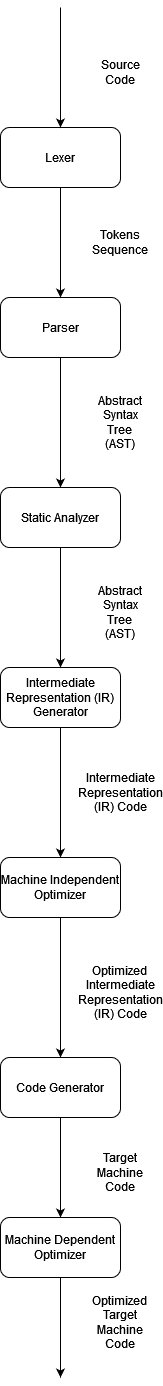
\includegraphics[width=\textwidth, height=0.8\textheight, keepaspectratio]{Figures/Arquiteturas/CompilersDetailedPipeline.png}  
  \caption{A detailed compiler structure}
  \label{fig:comp}
\end{figure}


It is also completely plausible to simplify this task by asking the students to implement a compiler that follows the following simplified structure:

\begin{figure}[H]  
  \centering
  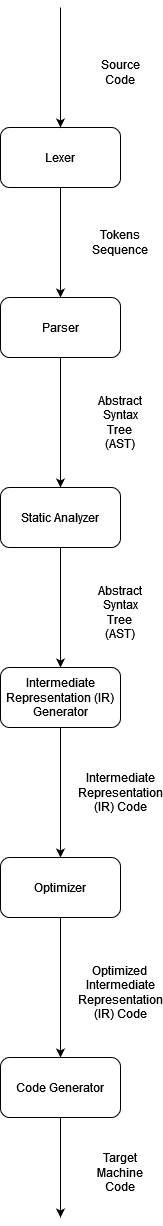
\includegraphics[width=\textwidth, height=0.8\textheight, keepaspectratio]{Figures/Arquiteturas/CompilersSimpliefiedPipeline.png}  
  \caption{A simplified compiler structure}
  \label{fig:Fluxograma}
\end{figure}
    
Section 2.4 is dedicated to provide an in-depth overview of each of the compiler's components from the simplified structure presented in the image above.


\section{What is an Interpreter and How Does it Distinguishes Itself From a Compiler?}
In order to explain what is an interpreter, it is necessary to recall the reader what is a compiler and what constitutes the compiling process.

A compiler is a program that takes as input a specific programming language and translates it to another, but without executing it. This step is delegated to the users, who must execute it by themselves.

In essence, compiling means translating code written in a source programming language to a target programming language (that is usually in a lower level, when compared to the source one). Whether the compiler generates machine code or bytecode, it is still performing a compiling process.

Once the reader has remembered what a compiler does and what compiling is, an interpreter is a program that takes as input a specific programming language and immediately executes it.

Keith Cooper and Linda Torczon provide another point of view to the discussion about the distinctions between compilers and interpreters in \cite{cooper2022engineering}.

According to them, a compiler is a type of software responsible for taking as input a program written in a certain source programming language and producing as output a representation of this very same program as a sequence of the instructions available at the target machine. Normally, the source programming language can be C, C++, Fortran, Java, and ML, while the "target" programming language is just the instruction set of a specific computer architecture (ARM, RISC-V, MIPS, x86, etc).

An interpreter, in contrast, receives as input a program written in a certain programming language, but its output is the result of executing the code written in the source language. Some language that fall into this category are: Perl and Scheme.

The images shown below are good examples that illustrate the input and the output of both compilers and interpreters:

\begin{figure}[H]  
  \centering
  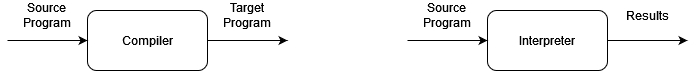
\includegraphics[width=\textwidth, height=\textheight, keepaspectratio]{Figures/Arquiteturas/Compilers and Interpreters.png}  
  \caption{Compilers and Interpreters}
  \label{fig:CompilersAndInterpreters}
\end{figure}

Finally, it is also highlight that there are some programming languages, such as Java and Python, whose implementations combine both compiling and interpreting. Considering Java as example, its implementation compiles the program written in the language to a bytecode format. Then, once the program is in the bytecode format, the Java Virtual Machine (JVM) executes the Java application (bytecode format) by running this bytecode inside the JVM (which can also be viewed as an interpreter for this lower-level representation). A similar process is followed by the Python programming language.

With this, it is reasonable to conclude that compilers and interpreters have a lot in common, due to the fact that they perform almost the same set of tasks, such as:
\begin{itemize}
    \item Analysis of the input program written in the source language in order to figure out if it is a valid one or not.
    \item Construction of internal models that are used to better understand the structure and meaning (semantics) of the input program.
    \item Determination of where to store values during the execution of the input program.
    
\end{itemize}

\section{Detailed Overview of Compiler's Components}

\subsection{Lexer}
The lexer is the first component present in the compiling process of a compiler. It is responsible for executing a process called lexing, which is also known as lexical analysis.

As earlier elucidated, the input of a compiler is the source code of a program written in a specific programming language. The content present inside the source code is viewed by the compiler as a large string, a linear sequence of characters, that has no meaning for it at all at this stage. The lexer's goal is to transform this sequence of characters that is the source code into a new representation that is more abstract from the compiler's perspective, so it can be passed on to the next component, the parser.

To perform such procedure, the lexer takes in this stream of characters and group them together forming a sequence of entities that convey the idea of a "word". These entities are called tokens.

Making an analogy to linguistics, one can say that the lexer's purpose is to group letters (characters) into words (tokens). Given this analogy, it is essential to inform the reader that, like words, tokens can have different lengths and different meanings. Some examples are listed below to better illustrate a few cases:
\begin{itemize}
    \item Single-Character Tokens: \texttt{(}, \texttt{\{}, \texttt{+}, \texttt{-}, \texttt{*}, \texttt{/}, etc.
    \item Double-Character Tokens: \texttt{==}, \texttt{!=}, \texttt{>=}, \texttt{<=}, etc.
    \item Multi-Character Tokens: \texttt{123} (a number literal), \texttt{"hello"} (a string literal), \texttt{true} (a boolean literal), \texttt{aVariable} (an identifier), etc.
\end{itemize}

It is also important to mention that certain characters have no meaning for the lexer during the lexical analysis and, therefore, are completely ignore in the process, such as: whitespace characters and characters that represent comments in the programming language in which the source file was written.

By the end of the lexical analysis, the sequence of characters is transformed into a sequence of tokens by following the syntax rules of the source programming language.

The figure below shows, in an simple example, the input and the output of this component:

\begin{table}[H]
    \centering
    \begin{tabular}{|c|c|c|c|c|c|c|c|c|c|c|c|c|c|c|c|c|c|c|c|c|}
        \hline
        l & e & t &  & a & v & g &  & = & ( & m & i & n & + & m & a & x & ) & / & 2 & ; \\
        \hline
    \end{tabular}
\end{table}

\begin{figure}[H]
  \centering
  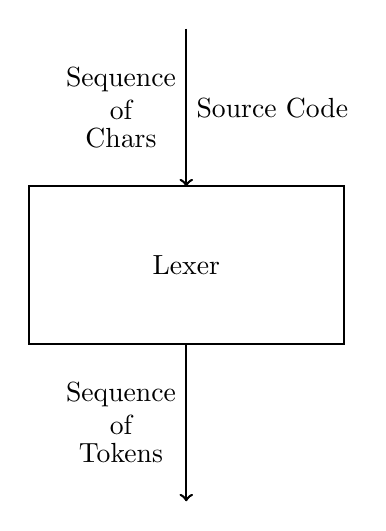
\begin{tikzpicture}
    % Draw the boxes
    \draw[thick] (0, 0) rectangle (4, 2);
    
    % Labels inside the boxes
    \node at (2, 1) {Lexer};

    % Input and output arrows
    \draw[->, thick] (2, 4) -- (2, 2) node[midway, left] {\shortstack{Sequence\\ of\\ Chars}};
    \draw[->, thick] (2, 4) -- (2, 2) node[midway, right] {\shortstack{Source Code}};
    \draw[->, thick] (2, 0) -- (2, -2) node[midway, left] {\shortstack{Sequence\\ of\\ Tokens}};
    \draw[->, thick] (2, 0) -- (2, -2) node[midway, left] {\shortstack{ }};
  \end{tikzpicture}
\end{figure}

\begin{table}[H]
    \centering
    \begin{tabular}{|c|c|c|c|c|c|c|c|c|c|c|}
        \hline
        let & avg & = & ( & min & + & max & ) & / & 2 & ; \\
        \hline
    \end{tabular}
\end{table}

\begin{figure}[H]  
  \caption{Input and Output of a Lexer}
  \label{fig:lexer}
\end{figure}

As seen in the example above, the lexer receives a sequence of characters, which represents the raw source code, and gives as the result a series of chunks of characters called tokens. Making another analogy with linguistics, one can think of tokens as the "words" and  the "punctuation" that constitutes a programming language.

Going further, it is also possible to say that the lexer's job is execute a traversal through the sequence of characters received and group such characters into the smallest sequences that represent something in the source programming language. Each of these resulting sequences of grouped characters is called a lexeme.

Therefore, in the example presented above, the sequence of lexemes produced from analyzing the sequence of characters received as input was: \texttt{let}, \texttt{avg}, \texttt{=}, \texttt{(}, \texttt{min}, \texttt{+}, \texttt{max}, \texttt{)}, \texttt{/}, \texttt{2}, \texttt{;}

In conclusion, lexemes are just raw substrings presented in the source code.

However, a token is much more than a lexeme. It generally contains other pieces of information that are useful in further stages of the compiling process and also in error report.

Usually, each token has a token type associated. For example, the lexeme \texttt{2} usually has \texttt{NUMBER} as its token type, while \texttt{+} often has \texttt{PLUS} as its token type. In this context, it is relevant to highlight that the amount of token types in a programming language basically depends on the amount of keywords (reserved words) that the language has, the amount of operators at the user's disposal, possibilities of literal values of different data types and, finally, the quantity of delimiters and separators.

Certain types of lexemes have literal values associated with them. numbers, booleans and strings, for example, fall into this category. In these cases, the lexer is able to convert the textual representation of the value into the living runtime entity that might be used by the compiler on later stages of the compiling process.

Last but not least, a compiler must also report errors when it encounters a lexical error during the lexing process, such as: an invalid number literal, an unterminated string, an invalid character that does not follow certain rules of the programming language. In order to report these errors, it is desired that the compiler display as much information as possible to the user about what went and, most importantly, where things went wrong. Having this in mind it is essential to store information about the location of each lexeme in the source code (the line it has appeared and, if possible, its column also).

Now it is time to analyze the functioning of a lexer from an implementation perspective.

The main part of a lexer's code is a loop and variables that are used as "pointers" to keep track of the beginning and ending of each lexeme present in the raw source code file. The lexer then starts working at the first character from the source code and, by using the mentioned "pointers" along with the lexical rules of the source programming language. For the reader that may not be familiar with it, the term "lexical rules" denotes a set of rules that define how characters are grouped to form lexemes in a programming language .Then, it discovers to which lexeme the current character belongs to and consumes any other following characters that also are part of the lexeme. When the end of such lexeme is found, information about its location and literal value are generated and grouped along with the lexeme in order to build and yield the token itself.

This process starts again, in the next iteration of the loop, at the first character that has not been consumed in the generation of the previous token and continues to traverse the source code and generate the corresponding tokens. The lexer continues to do this until it reaches the end of the file. When this happens, it sends the sequence of produced tokens to the next component of the compiler, the parser.

And that is it for lexers. As explained above its implementation is fairly simple and can be done by the programmer without much trouble. In spite of that, it is possible to delegate this task to certain tools, such as: Lex \cite{lesk1975lex} and Flex \cite{Flex}. For the sake of exposition and learning, they work in the following way:

\begin{enumerate}
    \item \textbf{Rule Writing:} When using such tools, the first step is to write the acceptable patters of characters of the source programming language through the use of regular expressions. These regular expressions define the lexemes that are useful and will be used to generate tokens. One example of rule could be "A sequence of digits must be treated as an integer number."
    
    \item \textbf{Lexer Generation and Execution in the C programming language:} Once the rules mentioned in the previous step have been written, the user can run Lex/Flex and the output will be a C program, the lexer that scans the input source code, identifies lexemes and generates the corresponding tokens based on the rules provided.
    
\end{enumerate}

\subsection{Parser}
The Parser is the second component present in the compiling process of a compiler. Its job is receive the sequence of tokens generated by the lexer in the previous stage, analyze if the provided sequence of tokens is valid or not by following the syntax rules of the source programming language, the Context-Free Grammar (CFG) and, finally, generating a new representation of the user's source code called Abstract Syntax Tree (AST). It can be said that, while the lexer performs a lexical analysis, the parser performs syntax analysis.

Going further, this component executes this transformation between the two mentioned representations of an user's code by performing two tasks simultaneously: While the parser is analyzing whether the received token stream represents a valid source code or not through the inspection of the source language's CFG, it also starts generating an hierarchical structure that resembles the idea of "traversing" a CFG. This hierarchical structure is called AST and each of its nodes represent a different construct of the source programming language. Examples of constructs are: variable declaration statements, if statements, loop statements, expressions, function declarations, and many others. In general, it is safe to say that the amount of node types depends on the expressiveness and amount of features of the source programming language.

Therefore, the core roles of a parser can be summarized as shown below:
\begin{itemize}
    \item \textbf{Syntax Verification:} The parser must guarantee that the received sequence of tokens is following the rules of the source language's CFG.
    
    \item \textbf{AST Building:} It also needs to build this tree representation of the source code, which is based on the token stream yielded by the lexer and the CFG rules. This newly formed tree representation is responsible for representing the syntactical constructs of the input program.
    
    \item \textbf{Error Reporting:} Finally, the parser is supposed to report any occurrences of syntax errors that might be found during the parsing process, so the user can correctly identify and fix them.

\end{itemize}


When it comes down to the implementation of this component, there two main classes of techniques responsible for grouping different algorithms that employ different ideas. Such classes are commonly called Top-Down and Bottom-Up:
\begin{itemize}
    \item \textbf{Top-Down:} The techniques that are in this category function with the same principle: Start the parsing process from the topmost rule present in the CFG of the source programming language and attempt to break down the input (token stream) into smaller substructures, by following the CFG rules.
        \begin{itemize}
            \item \textbf{Recursive Descent parsing:} This technique is considered to be the most simple and intuitive one compared to all the others presented here. Nevertheless, it is relevant to mention recursive descent parsers are fast, robust and can handle error reporting very well. Furthermore, according to Nystrom in \cite{nystrom2021crafting}, this technique is applied in several famous programming language implementations, such as: GCC, V8 (Google Chrome's JavaScript Runtime) and Roslyn (Microsoft's C\# compiler written in C\#).
            
            Since it is a technique that belongs to the Top-Down class of parsing techniques, this approach starts the parsing procedure from the topmost (or outermost) rule from the source language's CFG. Then, it starts "traversing" the CFG, navigating through subexpressions all the way down until it reaches the leaves of the AST (that is, until it reaches a sequence only composed of tokens or it finds a syntax error).

            The simplicity and intuitiveness of the recursive descent parsing comes from the fact that when implementing it, every rule of the language's CFG becomes a function and the body of the rule can be easily translate into code as shown in the table below:

            \begin{table}[h!]
                \centering
                \begin{tabular}{|c|c|}
                    \hline
                    \textbf{Grammar notation} & \textbf{Code representation} \\
                    \hline
                    Non-Terminal Symbol & Call to the function that represents that rule \\
                    Terminal Symbol & Code to match and consume a token \\
                    \texttt{|} & \texttt{if}, \texttt{switch} statement  \\
                    \texttt{*}, \texttt{+} & \texttt{for}, \texttt{while} loop \\
                    \texttt{?} & \texttt{if} statement \\
                    \hline
                \end{tabular}
                \caption{Translation between CFG's notation and its equivalent code implementation.}
            \end{table}

            The "recursive" term in recursive-descent parsing comes from the fact that if the non-terminal symbol of a rule's head is also present in the same rule's body, then when the translation to code happens, recursive function calls will happen depending on the source code provided as input to the compiler.

            Its advantages are the easiness and simplicity to implement it by hand and, due to that it is an excellent option to deal with programming languages that have simple CFGs and also for educational purposes.

            On the other hand, its disadvantages are the fact that it cannot handle left-recursive CFGs (those which have rules where non-terminal refers to itself at the start of the same rule) and it can become increasingly more complex to extend and maintain as the CFG of the programming language becomes larger and more complex.


            \item \textbf{LL parsing:} This technique is considered to be more methodical when compared to the previous one. Such approach reads the token stream from left to right and produces a leftmost derivation of the input by using K tokens of lookahead. Thus, if a parser is called LL(1), then it means that it has 1 token of lookahead. If it is LL(2), it has 2, and so on.
            
            The advantages of this procedure is that it is predictive parsing, hence there is no need to execute backtracking, which would slow down the parsing process as a whole, and it is more than enough to deal with programming languages whose grammars are simple and have no left-right recursion, which makes it a good candidate when implementing a project for a Compilers course at college.

            The disadvantages of it is that this technique is, unfortunately, limited to CFGs that are LL(k). Which means that, in these scenarios, there is a necessity of first rewriting the grammar to be LL(k) and, only then, implementing the parser itself with this approach.
        \end{itemize}
    \item \textbf{Bottom-Up:} The techniques that are in this category function with the same principle: Start the parsing process by examining the received token stream and trying to construct the AST by working from the terminal symbols of the language's CFG all the way up to the start symbol of the topmost CFG rule.
        \begin{itemize}
            \item \textbf{LR parsing:} This technique is very similar to the previously explained LL parsing. It starts out by processing the received sequence of tokens from left to right, however it produces at rightmost derivation (instead of the leftmost one) in reverse using K tokens of lookahead.

            The advantages of this procedure is that it is more robust and powerful when compared to LL parsing, due to the fact that it can deal with a wider variety of CFGs, including those that are left-recursive. Moreover, such approach is considered to be a good choice when implementing machine-yielded parsers.

            The only downsides of this approach are the its complexity of implementation when compared to the Recursive-Descent and the LL approaches, and its defying nature when it comes to debugging.
            
        \end{itemize}
\end{itemize}

In \cite{nystrom2021crafting}, Nystrom mentions other exotic parsing techniques, such as: LALR parsing, SLR parsing, Earley parsers, Pratt parsing, packrat parsing, parser combinators and the Shunting-Yard algorithm.

There are also tools that automate the process of building a parser. A few examples are: ANTLR \cite{ANTLR}, Bison \cite{Bison} and Yacc \cite{Yacc}. All of these tools operate, in essence, in the same way, with a few peculiarities and twists for each one. Basically, they take the CFG of the source programming language as input and produces as output a parser that can recognize valid and invalid programs written in that language. Such tools are very useful because they automate the burdening process of writing a parser by hand, especially when dealing with large CFGs.

Lastly, in order to better illustrate what a parser does, the image below shows what the parser might generate for a very simple program:

First, consider the following sequence of tokens received from the lexer:

\begin{table}[H]
    \centering
    \begin{tabular}{|c|c|c|c|c|c|c|c|c|}
        \hline
        let & seven & = & 2 & * & 3 & + & 1 & ; \\
        \hline
    \end{tabular}
\end{table}

\begin{figure}[H]  
  \caption{Example of token sequence provided as input to the parser.}
  \label{fig:inputParser}
\end{figure}

The output generated by the parser would be something very similar to the following AST:

\begin{figure}[H]  
  \centering
  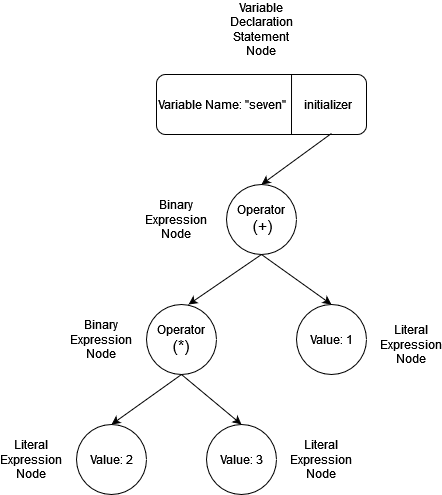
\includegraphics[width=0.6\textwidth, height=0.6\textheight, keepaspectratio]{Figures/Arquiteturas/ParserOutput.png}  
  \caption{Example of AST generated as output by the parser.}
  \label{fig:CompilersAndInterpreters}
\end{figure}

\subsection{Static Analyzer}
The Static Analyzer is the third component present in the compiling process of a compiler. It is responsible for performing a task called static analysis. Static analysis essentially means examining the source code without executing it, hence the name. Delving into it, the static analyzer's task is certify that the source code stick to correctness rules defined by the source programming language design and principles.

Such correctness rules include and are not limited to:
\begin{itemize}
    \item \textbf{Scope and Name Resolution:} This set of rules is responsible for ensuring that variables, functions and classes/types are declared before they are used. In addition, it is also in charge of making the correct bindings between an identifier use and its corresponding declaration, considering the scopes presented in the program's source code.
    
    \item \textbf{Type Checking:} Is an action performed by the static analyzer responsible for ensuring that functions, expressions and variables are properly used. For example: a value of type \texttt{int} cannot be multiplied by a value of type \texttt{bool}, if in a certain function with one parameters expects a value of type \texttt{string}, a value of type \texttt{int} cannot be passed as an argument in a call to such function.
    
    \item \textbf{Detection of Syntax Errors:} Although the parser is responsible for detecting such class of errors, some of these are easier detected during the static analysis stage. For example, a static analyzer can easily detect the misuse of the \texttt{return} keyword outside of a function (default or anonymous) or method. It can also detect the misuse of the \texttt{break} and \texttt{continue} keywords outside of loop statements. There are more examples related to these types of scenarios, but the two mentioned above are good and common examples.
    
    \item \textbf{Detection of Undeclared Variables and Functions:} As the rule's name suggests, a static analyzer is capable of recognizing the usage of variables and functions that have not been previously declared by the developer. It is also worth mentioning, that certain static analyzers take a step beyond and warn the user about variables and functions that have been declared but were never used in the program's source code.
\end{itemize}

Moreover, it is very important to remember the reader that the enforcement of such rules are performed on the Abstract Syntax Tree (AST) provided by the parser in the previous compiling stage, and the output of the static analyzer component is the same, the Abstract Syntax Tree (AST).

Finally, yet importantly, it is essential to highlight the fact that in mature compilers (Clang, GCC, javac, Roslyn, rustc, etc.) there is usually more than one static analyzer component where each one of them is responsible for receiving different representations of the program's source code and, consequently, enforcing different types of rules according to the philosophy of the source language.

For instance, there are static analyzers that are able to identify unused variables from just traversing the generated AST from the parser.

Last but not least, there are static analyzers that only operate on certain representations of the user's source code. Some static analyzers operate on Intermediate Representation (IR), which is a different type of representation of the source code. It is worth mentioning that this one is more abstract and it is designed to be easier to analyze compared to an AST as it removes details that are too specific of the source programming language. Analyzers that act on this type of representation can perform more complex analysis, such as Control Flow Analysis (whose focus is on detecting unreachable code and ensuring the non existence of infinite loops) and Data Flow Analysis (whose focus is on tracking how values flow between variables).

\subsection{Intermediate Representation (IR) Generator}
After the previous phases, it is time for the IR generator comes into play. This component receives as the AST from the Static Analyzer and transforms it into another representation of the user's source code that is generally closer to machine-code or bytecode, which, by consequence, makes it also closer to the hardware.

Before explaining with more details what an IR really is and how it works it is essential to remind the reader that the compiler is divided into two big components: the front-end (responsible for dealing with the source programming language) and the back-end (responsible for dealing with the target computer architecture).

Given this structure, there usually exist some kind of code representation that works as a bridge between the front-end and the back-end. Given this motivation, the IR normally is not tied neither to the source programming language and nor to the machine-code of the target architecture or bytecode. By using an IR to link the front and back-ends, the user can implement multiple compilers targeting different architectures with less effort.

The image below shows the huge different that the use of an IR generator component makes inside a compiler:

\begin{figure}[H]  
  \centering
  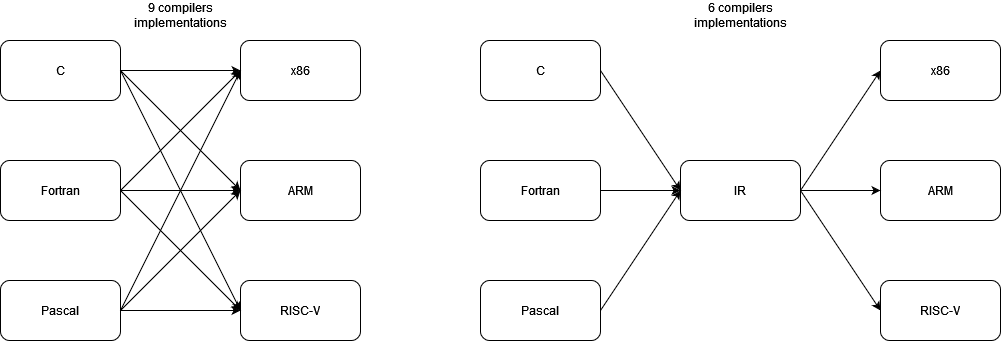
\includegraphics[width=\textwidth, height=\textheight, keepaspectratio]{Figures/Arquiteturas/IRImpact.png}  
  \caption{Impact of IR in multiple compilers implementations.}
  \label{fig:IRImpact}
\end{figure}

Basically, the developer implements only one front-end for each source language that produces the IR. Then only one back-end for each target architecture. Now, one is able to combine those to get every possible combination of source language and target architecture.

\subsection{Optimizer}
After the previous component emits the code in the intermediate representation (IR) format, it is time for the compiler to make the program more efficient in terms of execution time and memory usage without changing the meaning of the program (i.e., its semantics). For that purpose, the optimizer component comes in.

Before providing an overview of optimization techniques, it is important to inform the reader that this subfield of programming languages design and compilers implementation is still very active, with new discoveries and improvements being made in a regular basis. Therefore, this subsection will focus on the most well-known and popular optimization techniques.

Optimization techniques can be divided into two different groups: Machine-Independent Optimization Techniques and Machine-Dependent Optimization Techniques. The first group consists of techniques that can be applied to the user's program in the IR format, this is why they are called machine-independent. The second group is made of optimization techniques that require information about the target hardware architecture in order to be applied, hence the name machine-dependent.

Now, it is time to take a look at these two groups in more details:

\begin{itemize}
    \item \textbf{Machine-Independent Optimization Techniques:}
        \begin{enumerate}
            \item \textbf{Constant Folding:} This optimization consists of checking whether there is an expression in the code that always evaluate to the same value. If that is the case, then, the compiler can perform such evaluation at this stage and replace the code related of the expression with the computed resulting value.
            
            \item \textbf{Constant Propagation:} This technique is responsible for identifying constants in the code and then replacing the use of such constants with their respective values throughout the code.
            
            \item \textbf{Common Subexpression Elimination (CSE):} The aim of this optimization is identify expressions that are computed several times with the exact same operands inside the code and, then, replace all of them with a single computation, making the program faster by not requiring the computation of the same expression multiple times.
            
            \item \textbf{Dead-Code Elimination:} This optimization technique aims to eliminate code that has no effect on the behavior of the program, such as: declared variables that are not used and code placed after a \texttt{return} statement. 
            
            \item \textbf{Inlining:} This one's goal is to remove function calls from the program and include the body of the function where the call to such function was made. By doing this, the overhead related to a function call is reduced, making the program faster.
            
            \item \textbf{Loop Invariant Code Motion:} This optimization technique, as the name suggests, move operations that generate the same result in every iteration of a loop to the outside of it. By performing this action, redundant computations are eliminated, making the program run faster.
            
            \item \textbf{Strength Reduction:} Such optimization approach is responsible for replacing expensive operations, from a computation point of view, with cheaper ones that do not alter the program's behavior.
        \end{enumerate}
    \item \textbf{Machine-Dependent Optimization Techniques:}
        \begin{enumerate}
            \item \textbf{Instruction Scheduling:} This optimization consists of reordering instructions of a particular CPU architecture in order to make a better usage of its instruction pipeline and avoid possible stalls. This sort of optimization takes into account the latency of each instruction and also the availability of finite physical resources, such as registers.
            
            \item \textbf{Register Allocation:} This optimization is responsible for improving the assignment process of variables and produced temporary values to the limited amount of registers from a CPU. Since a CPU has a limited number of registers, this optimization tries to find out which variables and values should be kept in registers and which should be stored in memory, with the purpose of enhancing the performance of the program (it is worth remembering the reader that an access to a register is faster than the access to the memory). Therefore, it is essential to find out which variables and values are more used in the program and store them in registers instead of the memory.
            
            \item \textbf{Instruction Selection:} The goal of this optimization technique is, given the IR representation of the source code, choose the most efficient set of instructions from the target hardware architecture to perform the required operations.
            
            \item \textbf{Branch Prediction Optimization:} This optimization's objective is alter the code configuration in order to minimize the probability of a branch misprediction occurs. Normally, this is achieved by rearranging the code in such way that execution paths that are frequently executed are placed closer and also in a way that matches the CPU's prediction policy.
            
            \item \textbf{Vectorization:} This technique's purpose is convert scalar instruction into vector instructions in order to leverage the SIMD (Single-Instruction, Multiple Data) capabilities of modern CPUs. By doing this, the execution time of the user's program is usually reduced.
        
        \end{enumerate}
\end{itemize}

Finally, as seen above, there are two different groups of optimizations that a compiler can perform. Therefore, it is very common that the pipeline of a compiler has two different optimizers, one right after the IR Generator (that deals with machine-independent optimizations) and another right after the Code Generator (responsible for machine-dependent optimizations).

\subsection{Code Generator}
Once the compiler has performed the machine-independent optimizations to the adopted IR, it is time to generate code for the target CPU architecture. This task is executed by the Code Generator component.

In this context, it is important to highlight to the reader that the generated code is just Assembly code of a specific hardware architecture, whether it is x86, ARM, MIPS, RISC-V or another.

When it comes down to the implementation of this component, two possible paths can be taken by the implementer: one can generate code for an existing architecture, that is a real CPU, or for a virtual one.

If the first way is taken, then the compiler generates machine code for a real CPU and, after that, an executable is yielded and, finally, can be load into the memory of the system by the operating system. The advantage of this approach is that the native code generated is extremely fast since it leverages the most of the architecture that it is targeting. However, the downsides might be intimidating, in order to achieve such speed, one often needs to have a deep knowledge about the architecture that the implemented compiler has selected. Also, once the selection is made, the compiler is tied to such architecture. This means that, if the compiler targets the RISC-V architecture, then it cannot work on a x86 or ARM device.

According to \cite{nystrom2021crafting}, as a mean to deal with these disadvantages, Martin Richards and Niklaus Wirth developed their compilers to generate code for a virtual machine, instead of a real one. In practice, this means that their compilers produced code for an hypothetical and idealized machine rather than for a specific real CPU chip.

Advancing into this topic, the intention behind designing these synthetic instructions of a virtual machine is very clever: It allows the compiler developer to create instructions that are linked to the semantics of the source programming language without needing to worry about the peculiarities of any CPU architecture.


\subsection{Virtual Machines}
As seen above, a virtual machine is one of the possible approaches when it comes to the code generation phase of a compiler.

If the developer has chosen to built a compiler that emits bytecode, then there is still one task left to be done. Since, the compiler yields bytecode, no CPU architecture is able to understand what this representation actually means.

In this case, there are two options available again:
\begin{itemize}
    \item Implement a "mini-compiler" that performs a translation between the generate bytecode and the target machine architecture. In this scenario, it is important to pay attention to two facts: First, the produced bytecode will be essentially acting as a sort of intermediate representation since a translation between it and the target chip will need to happen. Second, the developer is again tied to the underlying hardware architecture. For each computer architecture, a new "mini-compiler" will have to be constructed.
    
    \item Implement a Virtual Machine (VM). In simple words, this is a program that emulates a chip that is able to fully understand the bytecode generated by the compiler. As one can already infer, virtual machines have their own trade-offs. Executing bytecode in a virtual machine is slower than directly executing native code in a computer architecture, due to the fact that each bytecode instruction must be simulated in software every time it executes instead of being executed by the hardware itself. On the other hand, by implementing a virtual machine, one gains a lot in terms of simplicity and portability. The need to translate the bytecode generated by the compiler to the machine code of a certain architecture is eliminated and say that the virtual machine was implemented in C or C++, then the implemented programming language can run in any platform that has a C or C++ compiler installed in it.
\end{itemize}


\subsection{Runtimes}
If the developer has opted to make the code generator directly produce machine code for a certain computer architecture, then the last step is tell the underlying operating system of the computer to load the executable file in the memory and execute it.

On the other hand, if the developer has opted to make the code generator yield bytecode, than the last step is start up the virtual machine, send the generated bytecode to it and execute the VM program.

In both of the mentioned cases, there is usually a need to have an environment that whose responsibility is provide support while the program has started its execution. Such piece of software is an essential part of the programming language implementation called Runtime.

The amount and type of responsibilities assigned to a runtime often varies according to the nature of the implemented programming language. However, some responsibilities are the same across different types of 
programming languages:

\begin{itemize}
    \item Interface with the Operating System.
    \item Memory Management.
    \item Execution of Built-In Functions.
    \item Process and Thread Management.
    \item Type Checking (for Dynamically-Typed Languages).
\end{itemize}


\section{Shortcuts and Alternate Routes}
This section is dedicated to present an overview of a few alternate ways of implementing a programming language besides the structured route exposed in the previous section. 

This is by no means an exhaustive list of possible approaches to be taken. Instead, it provides an overview of the most common and simple ones.

\subsection{Single-Pass Compilers}
A single-pass compiler is simple type of compiler that operates by interleaving the parsing, static analysis and code generation steps inside the parser component in order to generate the output code.

These kinds of compilers function without ever needing to use an AST or another sort of IR.

This simplicity, however, comes with a cost. The language design becomes severely restricted due to the way a single-pass compiler works. The developer does not have any kind of data structure to store information about the program and once some part of the code is parsed, it won't be re-visited later on, hence the name single-pass compiler. Essentially, this means that every time a statement or expression is parsed, the compiler needs to have enough information in order to correctly compile it.

The technique that enables single-pass compilers is known as "syntax-directed translation". In this approach, the developer establishes a link between a component of the programming language's grammar, one that outputs code, and an action to be executed. Then, when the parser starts its job, as soon as it identifies a piece of grammar that has an action associated, it executes such action, emitting the output code, step by step.

According to \cite{nystrom2021crafting}, both C and Pascal were firstly designed with the mentioned limitation in mind. It is worth remembering the reader that, at the time of these languages' conception, memory was very scarce. At certain times, compilers were not even able to deal with a single source file, let alone an entire program.

\subsection{Tree-Walk Interpreters}
A tree-Walk interpreter is a simple kind of interpreter that usually works by executing code right after the parser generates the AST.

In this scenario, a tree-walk interpreter runs the user's source code by executing a traversal on the received AST and performing different types of actions by taking into account the type of node that it is currently on.

Due to its simplicity, this kind of programming language implementation is very common in student projects and toy languages. However, it is not often used in general-purpose language, since the nature of the code execution makes it slow, with one exception, according to \cite{nystrom2021crafting}, being the earlier versions of Ruby, which were implemented as tree-walk interpreters up to version 1.9, when the language implementation was changed to a bytecode virtual machine.

\subsection{Transpilers}
A transpiler, also known as source-to-source compiler or transcompiler, is special type of compiler. The idea behind it is very simple: Instead of translating the program written in a source programming language to some kind of intermediate representation (AST, IR, CFG, etc), it translates the program to another source programming language.

Going further into its functioning, the developer writes the front-end components of a compiler as usual. Nevertheless, in the compiler's back-end, the programmer generates a string of valid code in another programming language that is as high-level as the source language, while preserving the meaning and semantics of the original program.

Finally, the programmer can use the compiler for the chosen high-level target language in order to delegate the heavy lifting of the back-end stage to this compiler. 

One of the most common use cases of a transpiler occurs in the context of web browsers. Nowadays, JavaScript is, by far, the most common choice to run code in it. However, JavaScript might not provide the best coding experience from certain developers' point of view. Due to that, a growing increase in the number of transpilers that have JavaScript as their target language has been observed, as can be seen in \cite{coffeescriptCompileToJS}.
